%%%%%%%%%%%%%%%%%%%%%%%%%%%%%%%%%%%%%%%%%
% Beamer Presentation
% LaTeX Template
% Version 1.0 (10/11/12)
%
% This template has been downloaded from:
% http://www.LaTeXTemplates.com
%
% License:
% CC BY-NC-SA 3.0 (http://creativecommons.org/licenses/by-nc-sa/3.0/)
%
%%%%%%%%%%%%%%%%%%%%%%%%%%%%%%%%%%%%%%%%%

%----------------------------------------------------------------------------------------
%	PACKAGES AND THEMES
%----------------------------------------------------------------------------------------

\documentclass{beamer}


\mode<presentation> {
	
	% The Beamer class comes with a number of default slide themes
	% which change the colors and layouts of slides. Below this is a list
	% of all the themes, uncomment each in turn to see what they look like.
	
	%\usetheme{default}
	%\usetheme{AnnArbor}
	%\usetheme{Antibes}
	%\usetheme{Bergen}
	\usetheme{Berkeley}
	%\usetheme{Berlin}
	%\usetheme{Boadilla}
	%\usetheme{CambridgeUS}
	%\usetheme{Copenhagen}
	%\usetheme{Darmstadt}
	%\usetheme{Dresden}
	%\usetheme{Frankfurt}
	%\usetheme{Goettingen}
	%\usetheme{Hannover}
	%\usetheme{Ilmenau}
	%\usetheme{JuanLesPins}
	%\usetheme{Luebeck}
	%\usetheme{Madrid}
	%\usetheme{Malmoe}
	%\usetheme{Marburg}
	%\usetheme{Montpellier}
	%\usetheme{PaloAlto}
	%\usetheme{Pittsburgh}
	%\usetheme{Rochester}
	%\usetheme{Singapore}
	%\usetheme{Szeged}
	%\usetheme{Warsaw}
	
	% As well as themes, the Beamer class has a number of color themes
	% for any slide theme. Uncomment each of these in turn to see how it
	% changes the colors of your current slide theme.
	
	%\usecolortheme{albatross}
	%\usecolortheme{beaver}
	%\usecolortheme{beetle}
	%\usecolortheme{crane}
	%\usecolortheme{dolphin}
	%\usecolortheme{dove}
	%\usecolortheme{fly}
	%\usecolortheme{lily}
	%\usecolortheme{orchid}
	%\usecolortheme{rose}
	%\usecolortheme{seagull}
	\usecolortheme{seahorse}
	%\usecolortheme{whale}
	%\usecolortheme{wolverine}
	
	%\setbeamertemplate{footline} % To remove the footer line in all slides uncomment this line
	%\setbeamertemplate{footline}[page number] % To replace the footer line in all slides with a simple slide count uncomment this line
	
	%\setbeamertemplate{navigation symbols}{} % To remove the navigation symbols from the bottom of all slides uncomment this line
}

\usepackage{amsmath,amssymb}
\usepackage{bm}
\usepackage{copyrightbox}

\usepackage{array}
\usepackage{tikz}
\usepackage{adjustbox}
\usepackage{ragged2e}
\usepackage{etoolbox}
\usepackage{subfigure}



\usepackage{graphicx} % Allows including images
\usepackage{booktabs} % Allows the use of \toprule, \midrule and \bottomrule in tables
\usepackage{bibentry}
%\usepackage[backend=biber,style=ieee, citestyle=authoryear]{biblatex}
%\usepackage[style=ieee-alphabetic, backend=bibtex]{biblatex}
\usepackage[style=numeric, backend=bibtex]{biblatex}



%\bibliography{bibfile.bib}
\addbibresource{bibfile.bib}



\makeatletter
\newcommand*{\mkblankfootnote}[1]{%
	\begingroup
	\renewcommand\thefootnote{}%
	\footnotetext{\bibfootnotewrapper{#1}}%
	\endgroup
}

\newcommand*{\mkbibsupercite}[1]{%
	\def\cbx@savedcites{\cbx@footfullcite}%
	\mkbibbrackets{#1}%
	\ifx\cbx@savedkeys\@empty
	\else
	\cbx@savedcites
	\fi}

\DeclareCiteCommand{\supercite}[\mkbibsupercite]
{\gdef\cbx@savedkeys{}}
{\usebibmacro{citeindex}%
	\usebibmacro{cite}%
	{}%
	\xappto\cbx@savedkeys{\thefield{entrykey},}}
{\supercitedelim}
{\protected@xappto\cbx@savedcites{%
		[\thefield{prenote}][\thefield{postnote}]{\cbx@savedkeys}}}

\DeclareCiteCommand{\cbx@footfullcite}
{}
{\mkblankfootnote{%
		\printtext[labelalphawidth]{%
			\usebibmacro{cite}%
		}%
		\setunit{\addspace}%
		\usedriver
		{\DeclareNameAlias{sortname}{default}}
		{\thefield{entrytype}}}}
{}
{}
\makeatother

\renewcommand*{\nameyeardelim}{\addcomma\addspace}

\apptocmd{\frame}{}{\justifying}{} % Allow optional arguments after frame.

\let\olditem\item
\renewcommand\item{\olditem\justifying}

\addtobeamertemplate{navigation symbols}{}{%
	\usebeamerfont{footline}%
	\usebeamercolor[fg]{footline}%
	\hspace{1em}%
	\insertframenumber/\inserttotalframenumber
}

%\makeatletter
%\@addtoreset{subfigure}{figure}
%\makeatother

%----------------------------------------------------------------------------------------
%	TITLE PAGE
%----------------------------------------------------------------------------------------

\definecolor{AtherosPrimary}{rgb}{0.992156,0.380392,0.34509803921}
\definecolor{AtherosSecondary}{rgb}{0.019,0,0.1568} % UBC Blue (primary)
\definecolor{AtherosTertiary}{rgb}{0.215,0.0625,0.515625}

\setbeamercolor{palette primary}{bg=AtherosSecondary,fg=white}
\setbeamercolor{palette tertiary}{bg=AtherosPrimary,fg=white}
\setbeamercolor{palette secondary}{bg=AtherosTertiary,fg=white}

\title{RIS-equiped Solar Panels} % The short title appears at the bottom of every slide, the full title is only on the title page

%\logo{\includegraphics[width=1.2cm,natwidth=212.6,natheight=212.6]{assets/sharif-logo.pdf}}
\logo{\includegraphics[width=1.2cm]{assets/sharif-logo.pdf}}


\author{Mohammad Raziei} % Your name
\institute[Sharif University] % Your institution as it will appear on the bottom of every slide, may be shorthand to save space
{
	Sharif University of Technology\\ % Your institution for the title page
	\medskip
	\textit{mohammadraziei1375@gmail.com} % Your email address
}
\date{\today} % Date, can be changed to a custom date

\graphicspath {{images/}}

\newcommand{\mypause}{\pause}

\begin{document}
	
	
	% Slide 1: Title Slide
	\begin{frame}
		\titlepage
	\end{frame}
	
	% Slide 2: Introduction
	
	\begin{frame}{Silicon is transparent to FR1-FR2}
		\begin{figure}
			\centering
			\copyrightbox[b]{
				\includegraphics[width=.7\linewidth]{images/ezgif-1-a1678707c9.jpg}
			}{\tiny\url{https://www.mdpi.com/1424-8220/24/22/7380}}
			\caption{
				\supercite{s24227380}
			}
		\end{figure}
		
	\end{frame}
	

	\begin{frame}{Solar cell structure}
		\begin{figure}
			\centering
			\subfigure[]{
				\copyrightbox[b]{
					\includegraphics[width=0.4\linewidth]{images/4e1060fb5850fa83e16134778b6961f0}
				}{\tiny\url{https://www.pinterest.com/pin/si-solar-cell-detail--422564377524497427/}}
			}
			\hfill
			\subfigure[]{
				\copyrightbox[b]{
					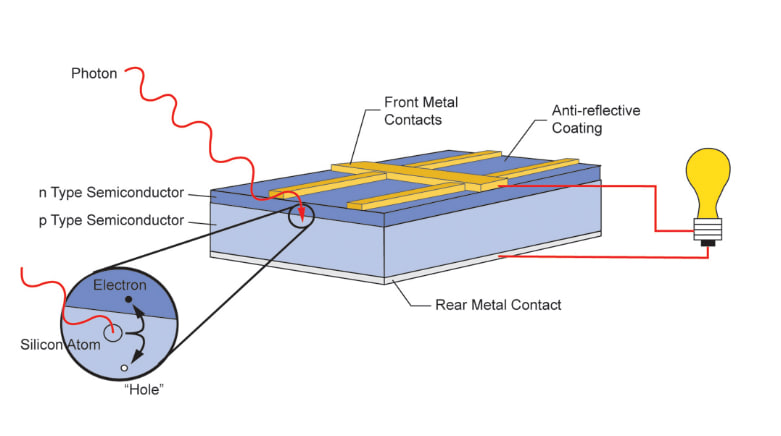
\includegraphics[width=0.45\linewidth]{images/photovoltaic}
				}{\tiny\url{https://www.viridiansolar.co.uk/resources-4-1-photovoltaic-effect.html}}
			}	
			\caption{Solar cell structure}
		\end{figure}
	\end{frame}
	
	
	\begin{frame}
		According to \supercite{Kerschaver2005}:
		\begin{figure}
			\centering
			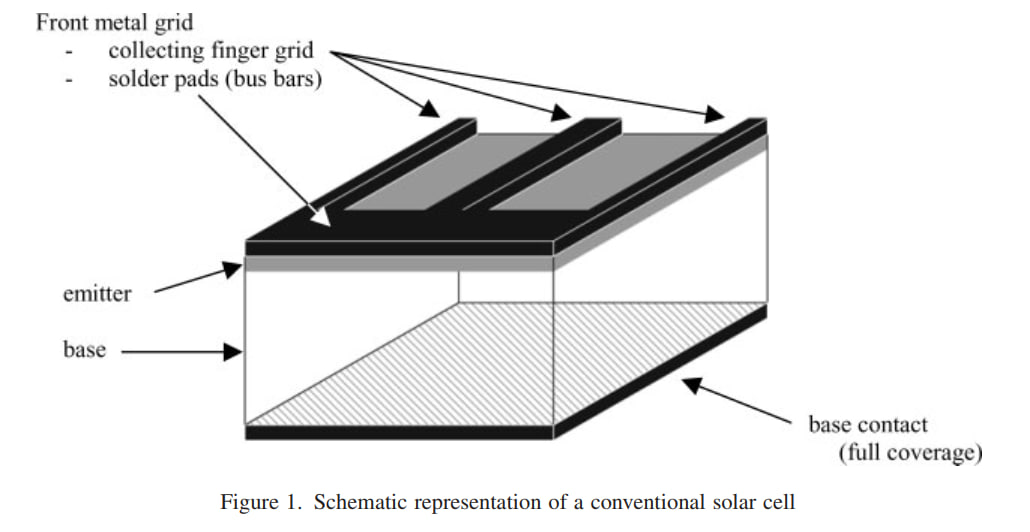
\includegraphics[width=0.7\linewidth]{images/auto-ris5}
			\caption{}
			\label{fig:auto-ris5}
		\end{figure}
	\end{frame}


\begin{frame}
	According to \supercite{Alhamad2024}
	\begin{figure}
		\centering
		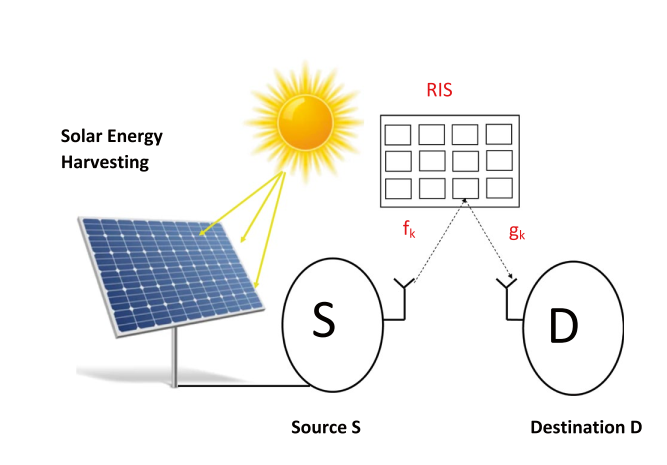
\includegraphics[width=0.7\linewidth]{images/auto-ris7}
		\caption{}
		\label{fig:auto-ris7}
	\end{figure}
	
\end{frame}



	\begin{frame}{Introduction}
		According to \supercite{Autonomous-RIS}:
		\begin{itemize}
			\item Transforming {Reconfigurable Intelligent Surfaces (RIS)} into eco-friendly, self-powered structures.
			\item \textbf{Challenges:}
			\begin{itemize}
				\item High power consumption of {RIS}.
				\item Trade-offs between antenna performance and energy harvesting.
			\end{itemize}
			\item \textbf{Solution:} Integration of high-efficiency {multi-junction (MJ)} solar cells with {RIS}.
		\end{itemize}
	\end{frame}
	
	% Slide 3: Background and Motivation
	\begin{frame}{Background and Motivation}
		\begin{itemize}
			\item \textbf{Reconfigurable Intelligent Surfaces (RIS):}
			\begin{itemize}
				\item Active metasurfaces with tunable components (e.g., varactor diodes).
				\item Controls phase and amplitude of electromagnetic waves.
			\end{itemize}
			\item \textbf{Motivation:}
			\begin{itemize}
				\item Reduce dependency on external power.
				\item Enable carbon-neutral, autonomous networks for remote and urban areas.
			\end{itemize}
		\end{itemize}
	\end{frame}
	
	
\begin{frame}
	\begin{figure}
		\centering
		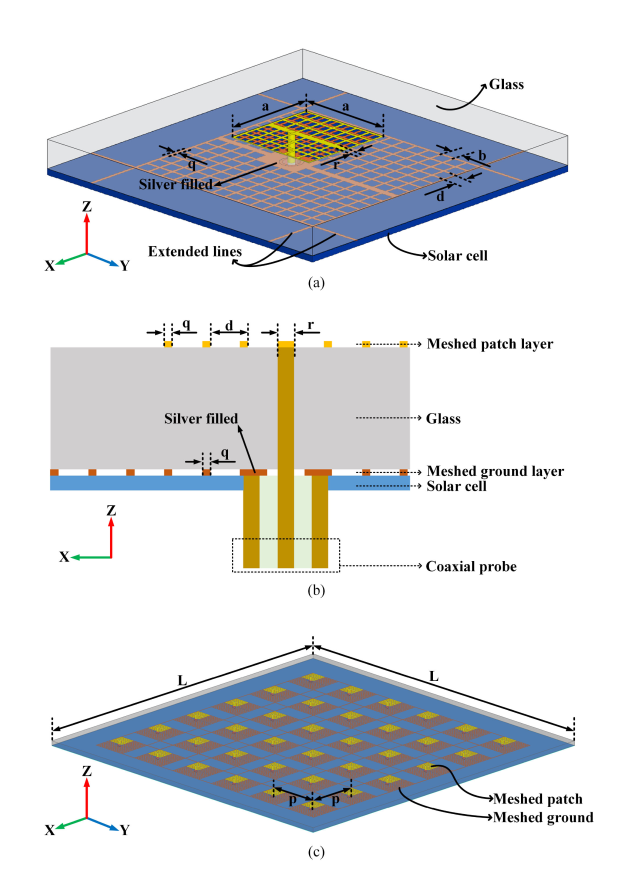
\includegraphics[width=0.3\linewidth]{images/auto-ris6}
		\caption{\supercite{OpticalTransparentAntennaArrayIntegratedWithSolarCell}}
		\label{fig:auto-ris6}
	\end{figure}
\end{frame}


	% Slide 5: Power Generation and Efficiency
	\begin{frame}{Power Generation and Efficiency}
		\begin{itemize}
			\item \textbf{Energy Harvesting:}
			\begin{itemize}
				\item Solar irradiance intensity far exceeds RF energy.
				\item \textbf{Modeling Results:}
				\begin{itemize}
					\item Sub-6GHz {RIS}: Solar cells generate $>$20 W of power under typical conditions.
					\item Battery backup: Must last three days without sunlight.
				\end{itemize}
			\end{itemize}
			\item \textbf{Design Optimization:}
			\begin{itemize}
				\item Use {MJ} solar cells with $>$30\% efficiency.
				\item Efficient {DC-DC} converters for power management.
			\end{itemize}
		\end{itemize}
	\end{frame}
	
	
	% Slide 4: Proposed Design Methodologies
	\begin{frame}{Proposed Design Methodologies}
		\textbf{Sub-6GHz RIS:}
		\begin{itemize}
			\item \textbf{Design:} Solar cells added between {RIS} unit cells in copper-free areas.
			\item \textbf{Key Dimensions:} Hybrid unit cell size = 40 mm, solar cell width = 18 mm.
			\item \textbf{Simulation Results:} Negligible impact on phase response for gaps $<$ 2 mm.
		\end{itemize}
		\textbf{5G mmWave RIS:}
		\begin{itemize}
			\item \textbf{Design:} Solar cell frame surrounding the {RIS}.
			\item \textbf{Advantages:}
			\begin{itemize}
				\item Reduced cost.
				\item Simple design integration.
			\end{itemize}
		\end{itemize}
	\end{frame}
	
	\begin{frame}
		\begin{figure}
			\centering
			\subfigure[FR1]{				
				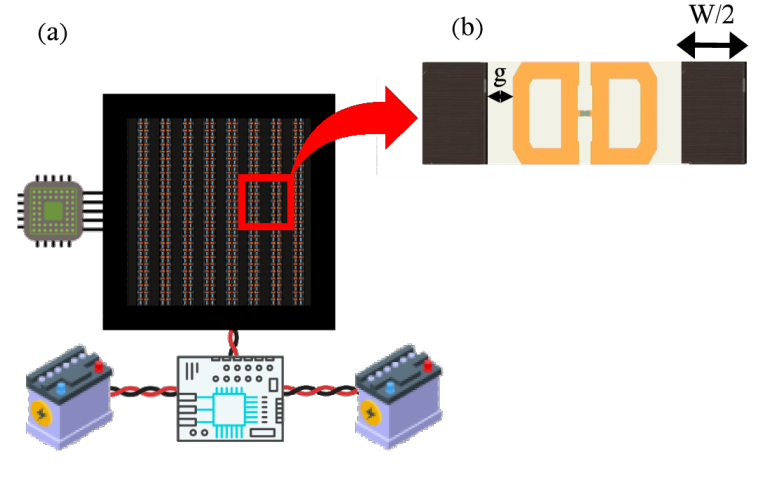
\includegraphics[width=0.5\linewidth]{images/auto-ris}
			}
			\hfill
			\subfigure[FR2]{
				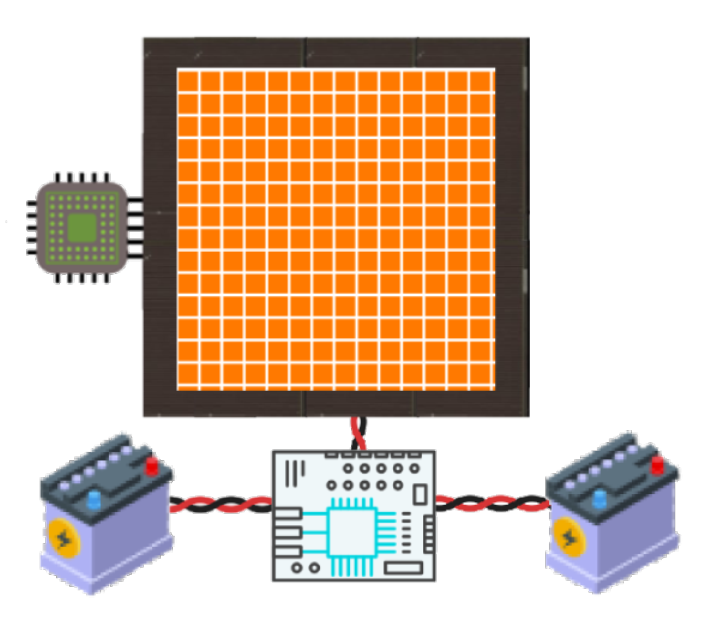
\includegraphics[width=0.4\linewidth]{images/auto-ris1}
			}
			\caption{\supercite{Autonomous-RIS}}
		\end{figure}
	\end{frame}
	
	\begin{frame}
		\begin{figure}
			\centering
			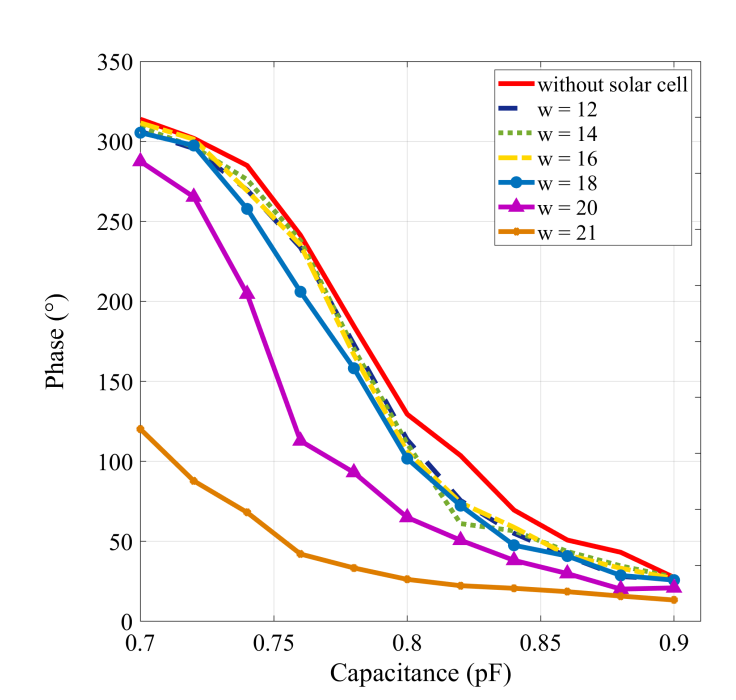
\includegraphics[width=0.7\linewidth]{images/auto-ris2}
			\caption{}
			\label{fig:auto-ris2}
		\end{figure}
	\end{frame}
	
\begin{frame}
	\begin{figure}
		\centering
		\subfigure[]{		
			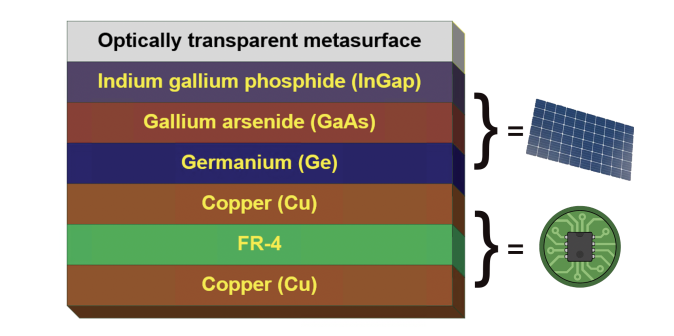
\includegraphics[width=0.5\linewidth]{images/auto-ris3}
		}
		\hfill
		\subfigure[]{		
			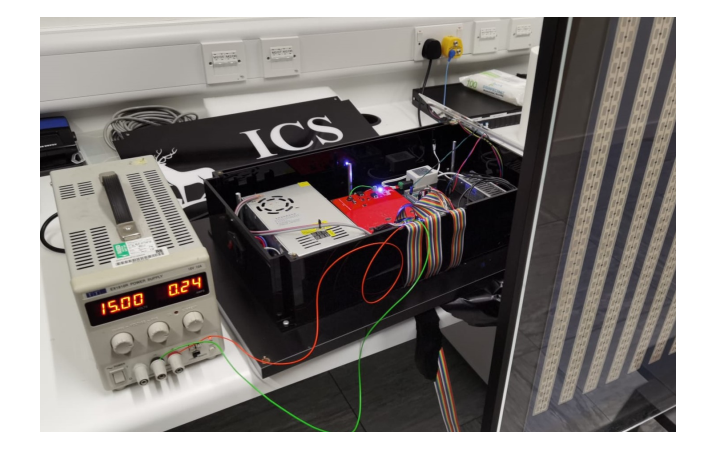
\includegraphics[width=0.4\linewidth]{images/auto-ris4}
		}
		\caption{}
		\label{fig:auto-ris4}
	\end{figure}

	
\end{frame}

\begin{frame}
	
	The authors of \supercite{9860773} analyse the energy harvesting model for RIS-assisted communications where the energy is harvested from radio waves.
	They concluded that the average
	power consumption of the RIS components must not exceed
	a few microwatts for the structure to become completely
	autonomous. 
	
	But the average power generated by
	photovoltaic cells exceeds 20 W in most cases \supercite{Autonomous-RIS}. 

\end{frame}
	
	% Slide 7: Future Directions
	\begin{frame}{Future Directions}
		\begin{itemize}
			\item \textbf{Improvements:}
			\begin{itemize}
				\item Enhance the power efficiency of {RIS} controllers.
				\item Develop low-power standby modes.
				\item Explore novel materials like 3D-printed solar cells.
			\end{itemize}
			\item \textbf{Applications:}
			\begin{itemize}
				\item Green communication systems for 5G, 6G, and beyond.
			\end{itemize}
		\end{itemize}
	\end{frame}
	
	% Slide 8: Conclusion
	\begin{frame}{Conclusion}
		\begin{itemize}
			\item \textbf{Summary:}
			\begin{itemize}
				\item Proposed designs demonstrate feasibility of integrating {MJ} solar cells into {RIS} for self-powering.
				\item Autonomous {RIS} structures pave the way for sustainable communication networks.
			\end{itemize}
			\item \textbf{Outlook:}
			\begin{itemize}
				\item Optimizing cost and scalability for industrial implementation.
			\end{itemize}
		\end{itemize}
	\end{frame}
	
	
	
	
	%----------------------------------------------------------------------------------------
	%-------------------                   References                     -------------------
	%----------------------------------------------------------------------------------------
	
	\begin{frame}[allowframebreaks]
		\frametitle{References}
		\printbibliography
	\end{frame}
	
	%----------------------------------------------------------------------------------------
	
\end{document} 

